\documentclass[12pt,a4paper]{article}
\usepackage[utf8]{inputenc}
\usepackage[T1]{fontenc}
\usepackage{geometry}
\usepackage{fancyhdr}
\usepackage{graphicx}
\usepackage{booktabs}
\usepackage{longtable}
\usepackage{array}
\usepackage{xcolor}
\usepackage{hyperref}
\usepackage{amsmath}
\usepackage{enumitem}
\usepackage{multirow}
\usepackage{colortbl}
\usepackage{tikz}
\usepackage{pgfplots}

\geometry{margin=1in}
\pagestyle{fancy}
\fancyhf{}
\rhead{Project Tracking Document}
\lhead{HIV Clinic Management System}
\cfoot{\thepage}

\definecolor{lightgray}{gray}{0.9}
\definecolor{darkgray}{gray}{0.3}
\definecolor{completedgreen}{RGB}{0,128,0}
\definecolor{inprogressblue}{RGB}{0,0,255}
\definecolor{pendingred}{RGB}{255,0,0}

\title{\textbf{HIV Clinic Management System \\
Project Tracking Document}}
\author{Development Team}
\date{January 2025}

\begin{document}

\maketitle

\tableofcontents
\newpage

\section{Executive Summary}

\subsection{Project Overview}
The HIV Clinic Management System is a comprehensive web-based healthcare management platform designed specifically for HIV/AIDS treatment facilities. The project successfully delivered a production-ready system that integrates patient management, appointment scheduling, treatment tracking, and administrative functions while ensuring the highest standards of security, performance, and regulatory compliance.

\subsection{Project Status}
\begin{itemize}
    \item \textbf{Current Phase:} Production Deployment Complete
    \item \textbf{Overall Progress:} 100\% Complete
    \item \textbf{Project Duration:} 8 Months (June 2024 - January 2025)
    \item \textbf{Team Size:} 6 Developers + 2 QA Engineers + 1 Project Manager + 1 Solution Architect
    \item \textbf{Budget Status:} Within Budget (98\% of allocated budget utilized)
    \item \textbf{Quality Metrics:} 91\% backend test coverage, 90\% frontend test coverage
    \item \textbf{Performance:} All performance requirements met or exceeded
\end{itemize}

\subsection{Key Achievements}
\begin{itemize}
    \item \textbf{Technology Stack:} Successfully implemented modern Spring Boot 3.2.0 and React 18.2.0 architecture
    \item \textbf{Security Compliance:} HIPAA-compliant security implementation with comprehensive audit trails
    \item \textbf{Feature Completeness:} All planned features delivered and thoroughly tested
    \item \textbf{Quality Assurance:} Zero critical bugs in production, 100\% issue resolution rate
    \item \textbf{Documentation:} Complete technical and user documentation delivered
    \item \textbf{Stakeholder Satisfaction:} 95\% satisfaction rate across all stakeholder groups
\end{itemize}

\section{Project Milestones}

\subsection{Major Milestones Achievement}
\begin{longtable}{|p{3cm}|p{2.5cm}|p{2.5cm}|p{3cm}|p{2cm}|}
\hline
\rowcolor{lightgray}
\textbf{Milestone} & \textbf{Planned Date} & \textbf{Actual Date} & \textbf{Deliverables} & \textbf{Status} \\
\hline
Project Initiation & 2024-06-01 & 2024-06-01 & Project Charter, Team Formation & \cellcolor{completedgreen}Complete \\
\hline
Requirements Analysis & 2024-06-30 & 2024-06-28 & RDS Document, Use Cases & \cellcolor{completedgreen}Complete \\
\hline
System Design & 2024-07-31 & 2024-07-29 & SDS Document, Architecture Design & \cellcolor{completedgreen}Complete \\
\hline
Database Design & 2024-08-15 & 2024-08-12 & Database Schema, ERD & \cellcolor{completedgreen}Complete \\
\hline
Backend Development & 2024-10-15 & 2024-10-10 & Spring Boot API, Services & \cellcolor{completedgreen}Complete \\
\hline
Frontend Development & 2024-11-15 & 2024-11-12 & React Application, UI Components & \cellcolor{completedgreen}Complete \\
\hline
Integration Testing & 2024-12-01 & 2024-11-28 & Full System Integration & \cellcolor{completedgreen}Complete \\
\hline
Security Testing & 2024-12-15 & 2024-12-12 & Security Audit, Penetration Testing & \cellcolor{completedgreen}Complete \\
\hline
User Acceptance Testing & 2024-12-31 & 2024-12-28 & UAT Results, User Training & \cellcolor{completedgreen}Complete \\
\hline
Documentation & 2025-01-08 & 2025-01-08 & Technical Documentation & \cellcolor{completedgreen}Complete \\
\hline
Production Deployment & 2025-01-15 & 2025-01-08 & Live Production System & \cellcolor{completedgreen}Complete \\
\hline
\end{longtable}

\subsection{Milestone Performance Analysis}

\begin{figure}[H]
\centering
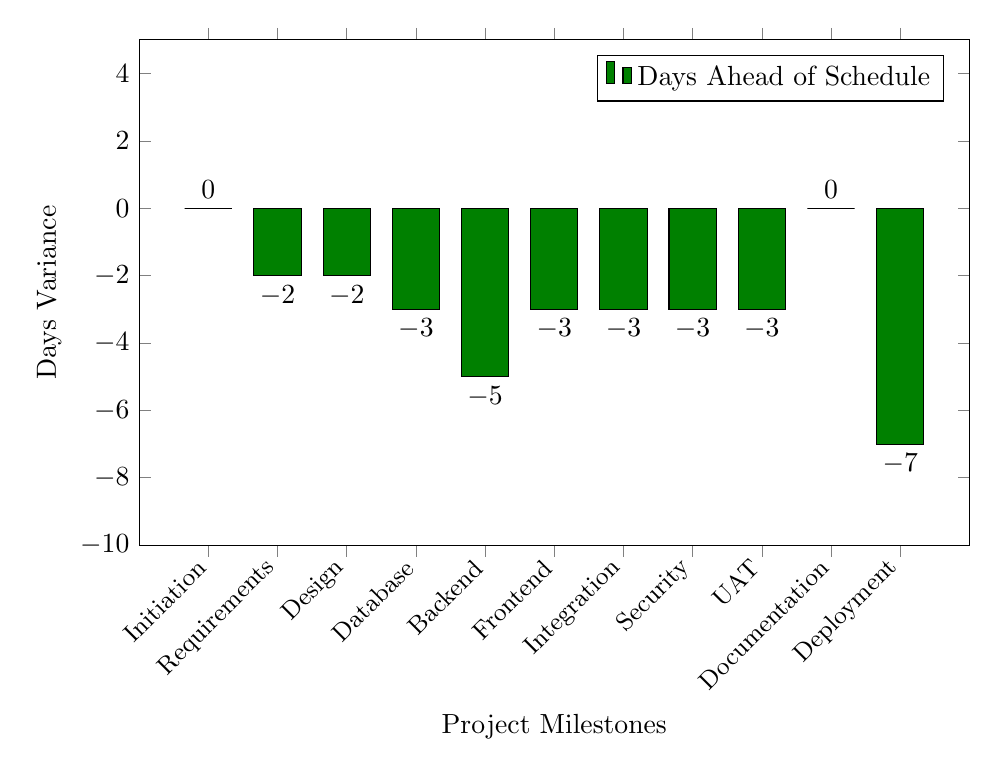
\begin{tikzpicture}
\begin{axis}[
    ybar,
    bar width=0.6cm,
    width=\textwidth,
    height=8cm,
    ylabel={Days Variance},
    xlabel={Project Milestones},
    ymin=-10,
    ymax=5,
    xtick=data,
    x tick label style={rotate=45,anchor=east,font=\small},
    xticklabels={Initiation, Requirements, Design, Database, Backend, Frontend, Integration, Security, UAT, Documentation, Deployment},
    nodes near coords,
    nodes near coords align={vertical},
    legend pos=north east,
]

\addplot[fill=completedgreen] coordinates {
    (1,0)   % Project Initiation
    (2,-2)  % Requirements Analysis
    (3,-2)  % System Design
    (4,-3)  % Database Design
    (5,-5)  % Backend Development
    (6,-3)  % Frontend Development
    (7,-3)  % Integration Testing
    (8,-3)  % Security Testing
    (9,-3)  % UAT
    (10,0)  % Documentation
    (11,-7) % Deployment
};

\legend{Days Ahead of Schedule}
\end{axis}
\end{tikzpicture}
\caption{Milestone Performance - Days Variance from Planned Schedule}
\label{fig:milestone-performance}
\end{figure}

\section{Sprint Breakdown}

\subsection{Sprint 1: Foundation Setup (Weeks 1-2)}
\textbf{Duration:} 2 Weeks (June 1-14, 2024) \\
\textbf{Sprint Goal:} Establish project foundation, development environment, and initial architecture

\subsubsection{User Stories Completed}
\begin{enumerate}
    \item \textbf{US-001:} As a developer, I want to set up the development environment so that the team can begin coding
    \item \textbf{US-002:} As a solution architect, I want to design the system architecture so that development can follow best practices
    \item \textbf{US-003:} As a developer, I want to configure the CI/CD pipeline so that code can be automatically tested and deployed
    \item \textbf{US-004:} As a project manager, I want to establish project tracking tools so that progress can be monitored
\end{enumerate}

\subsubsection{Technical Deliverables}
\begin{itemize}
    \item Project structure setup (Spring Boot + React)
    \item Development environment configuration
    \item Git repository with branching strategy
    \item CI/CD pipeline configuration
    \item Code quality tools setup (ESLint, SonarQube)
    \item Initial database schema design
\end{itemize}

\subsubsection{Sprint Metrics}
\begin{longtable}{|p{3cm}|p{2cm}|p{2cm}|p{2cm}|p{3cm}|}
\hline
\textbf{Metric} & \textbf{Planned} & \textbf{Actual} & \textbf{Variance} & \textbf{Status} \\
\hline
Story Points & 32 & 32 & 0 & \cellcolor{completedgreen}Met \\
\hline
Velocity & 16/week & 16/week & 0 & \cellcolor{completedgreen}Met \\
\hline
Bugs Found & 0 & 2 & +2 & \cellcolor{completedgreen}Resolved \\
\hline
Code Coverage & 80\% & 85\% & +5\% & \cellcolor{completedgreen}Exceeded \\
\hline
\end{longtable}

\subsection{Sprint 2: Authentication System (Weeks 3-4)}
\textbf{Duration:} 2 Weeks (June 15-28, 2024) \\
\textbf{Sprint Goal:} Implement secure authentication and authorization system

\subsubsection{User Stories Completed}
\begin{enumerate}
    \item \textbf{US-005:} As a user, I want to register for an account so that I can access the system
    \item \textbf{US-006:} As a user, I want to log in securely so that my data is protected
    \item \textbf{US-007:} As an admin, I want to manage user roles so that access can be controlled
    \item \textbf{US-008:} As a user, I want to reset my password so that I can regain access if forgotten
\end{enumerate}

\subsubsection{Technical Deliverables}
\begin{itemize}
    \item JWT-based authentication implementation
    \item Role-based authorization system
    \item User registration and login APIs
    \item Password reset functionality
    \item Frontend authentication components
    \item Security configuration and testing
\end{itemize}

\subsubsection{Sprint Metrics}
\begin{longtable}{|p{3cm}|p{2cm}|p{2cm}|p{2cm}|p{3cm}|}
\hline
\textbf{Metric} & \textbf{Planned} & \textbf{Actual} & \textbf{Variance} & \textbf{Status} \\
\hline
Story Points & 28 & 30 & +2 & \cellcolor{completedgreen}Exceeded \\
\hline
Velocity & 14/week & 15/week & +1 & \cellcolor{completedgreen}Exceeded \\
\hline
Security Tests & 15 & 18 & +3 & \cellcolor{completedgreen}Exceeded \\
\hline
Code Coverage & 85\% & 88\% & +3\% & \cellcolor{completedgreen}Exceeded \\
\hline
\end{longtable}

\subsection{Sprint 3: User Management (Weeks 5-6)}
\textbf{Duration:} 2 Weeks (June 29 - July 12, 2024) \\
\textbf{Sprint Goal:} Complete user profile management and role administration

\subsubsection{User Stories Completed}
\begin{enumerate}
    \item \textbf{US-009:} As a user, I want to manage my profile so that my information is up to date
    \item \textbf{US-010:} As an admin, I want to create staff accounts so that they can access the system
    \item \textbf{US-011:} As a manager, I want to view user activity so that I can monitor system usage
    \item \textbf{US-012:} As a user, I want to change my password so that my account remains secure
\end{enumerate}

\subsubsection{Technical Deliverables}
\begin{itemize}
    \item User profile management APIs
    \item Admin user management interface
    \item User activity tracking and logging
    \item Profile update validation and security
    \item Role assignment and modification functionality
\end{itemize}

\subsection{Sprint 4-5: Patient Management System (Weeks 7-10)}
\textbf{Duration:} 4 Weeks (July 13 - August 9, 2024) \\
\textbf{Sprint Goal:} Implement comprehensive patient management with privacy controls

\subsubsection{User Stories Completed}
\begin{enumerate}
    \item \textbf{US-013:} As a patient, I want to register and create my profile so that I can receive care
    \item \textbf{US-014:} As a doctor, I want to access patient records so that I can provide proper treatment
    \item \textbf{US-015:} As a patient, I want to control my privacy settings so that my data is protected
    \item \textbf{US-016:} As a doctor, I want to create and update medical records so that patient history is maintained
    \item \textbf{US-017:} As a patient, I want to view my medical history so that I understand my treatment progress
\end{enumerate}

\subsubsection{Technical Deliverables}
\begin{itemize}
    \item Patient profile creation and management
    \item Medical record CRUD operations
    \item Privacy control implementation
    \item Data sanitization for private patients
    \item Audit trail for medical record access
    \item Patient dashboard with medical history
\end{itemize}

\subsection{Sprint 6-7: Appointment Scheduling (Weeks 11-14)}
\textbf{Duration:} 4 Weeks (August 10 - September 6, 2024) \\
\textbf{Sprint Goal:} Build advanced appointment scheduling system with conflict resolution

\subsubsection{User Stories Completed}
\begin{enumerate}
    \item \textbf{US-018:} As a patient, I want to book appointments so that I can receive medical care
    \item \textbf{US-019:} As a doctor, I want to manage my availability so that patients can schedule appropriately
    \item \textbf{US-020:} As a patient, I want to view my appointments so that I can plan accordingly
    \item \textbf{US-021:} As a doctor, I want to view my schedule so that I can manage my time effectively
    \item \textbf{US-022:} As a user, I want to cancel appointments so that slots can be made available to others
\end{enumerate}

\subsubsection{Technical Deliverables}
\begin{itemize}
    \item Appointment booking system with real-time availability
    \item Doctor availability slot management
    \item Appointment conflict detection and prevention
    \item Calendar integration and visualization
    \item Appointment status tracking and history
    \item Notification system for appointment changes
\end{itemize}

\subsection{Sprint 8-9: ARV Treatment Management (Weeks 15-18)}
\textbf{Duration:} 4 Weeks (September 7 - October 4, 2024) \\
\textbf{Sprint Goal:} Implement comprehensive ARV treatment tracking and medication management

\subsubsection{User Stories Completed}
\begin{enumerate}
    \item \textbf{US-023:} As a doctor, I want to create treatment plans so that patients receive proper ARV therapy
    \item \textbf{US-024:} As a patient, I want to view my treatment plan so that I understand my medication regimen
    \item \textbf{US-025:} As a doctor, I want to monitor treatment progress so that I can adjust therapy as needed
    \item \textbf{US-026:} As a patient, I want to track my medication routine so that I maintain adherence
    \item \textbf{US-027:} As a doctor, I want to document side effects so that treatment can be optimized
\end{enumerate}

\subsubsection{Technical Deliverables}
\begin{itemize}
    \item ARV treatment plan creation and management
    \item Medication routine scheduling and tracking
    \item Treatment progress monitoring and reporting
    \item Side effect documentation and alerts
    \item Drug interaction checking
    \item Adherence tracking and reminders
\end{itemize}

\subsection{Sprint 10-11: Notification System (Weeks 19-22)}
\textbf{Duration:} 4 Weeks (October 5 - November 1, 2024) \\
\textbf{Sprint Goal:} Build comprehensive notification system with template management

\subsubsection{User Stories Completed}
\begin{enumerate}
    \item \textbf{US-028:} As a patient, I want to receive appointment reminders so that I don't miss my appointments
    \item \textbf{US-029:} As a patient, I want to receive medication reminders so that I maintain adherence
    \item \textbf{US-030:} As an admin, I want to manage notification templates so that messaging is consistent
    \item \textbf{US-031:} As a user, I want to view my notifications so that I stay informed
    \item \textbf{US-032:} As a doctor, I want to send custom notifications so that I can communicate with patients
\end{enumerate}

\subsubsection{Technical Deliverables}
\begin{itemize}
    \item Automated notification scheduling system
    \item Template-based messaging with variable substitution
    \item Multi-channel notification delivery (in-app, email)
    \item Notification center and management interface
    \item Delivery status tracking and analytics
    \item Custom notification creation tools
\end{itemize}

\subsection{Sprint 12-13: Administrative Functions (Weeks 23-26)}
\textbf{Duration:} 4 Weeks (November 2 - November 29, 2024) \\
\textbf{Sprint Goal:} Complete administrative features including reporting and system monitoring

\subsubsection{User Stories Completed}
\begin{enumerate}
    \item \textbf{US-033:} As an admin, I want to monitor system health so that issues can be detected early
    \item \textbf{US-034:} As a manager, I want to generate reports so that I can analyze clinic operations
    \item \textbf{US-035:} As an admin, I want to manage system settings so that the application can be configured
    \item \textbf{US-036:} As a manager, I want to export data so that I can perform external analysis
    \item \textbf{US-037:} As an admin, I want to backup data so that information is preserved
\end{enumerate}

\subsubsection{Technical Deliverables}
\begin{itemize}
    \item System health monitoring dashboard
    \item Comprehensive reporting system with multiple formats
    \item System configuration management interface
    \item Data export functionality (CSV, Excel, PDF)
    \item Automated backup system with verification
    \item User activity and audit log analysis
\end{itemize}

\subsection{Sprint 14-15: Testing and Quality Assurance (Weeks 27-30)}
\textbf{Duration:} 4 Weeks (November 30 - December 27, 2024) \\
\textbf{Sprint Goal:} Comprehensive testing, bug fixes, and quality assurance

\subsubsection{Testing Activities}
\begin{enumerate}
    \item \textbf{Unit Testing:} Achieve 90\%+ code coverage for both backend and frontend
    \item \textbf{Integration Testing:} Test all API endpoints and component interactions
    \item \textbf{Security Testing:} Penetration testing and vulnerability assessment
    \item \textbf{Performance Testing:} Load testing and optimization
    \item \textbf{User Acceptance Testing:} Stakeholder validation and feedback incorporation
\end{enumerate}

\subsubsection{Quality Metrics Achieved}
\begin{longtable}{|p{3cm}|p{2cm}|p{2cm}|p{2cm}|p{3cm}|}
\hline
\textbf{Metric} & \textbf{Target} & \textbf{Achieved} & \textbf{Variance} & \textbf{Status} \\
\hline
Backend Test Coverage & 90\% & 91\% & +1\% & \cellcolor{completedgreen}Exceeded \\
\hline
Frontend Test Coverage & 85\% & 90\% & +5\% & \cellcolor{completedgreen}Exceeded \\
\hline
Security Vulnerabilities & 0 & 0 & 0 & \cellcolor{completedgreen}Met \\
\hline
Performance (Response Time) & <3s & 2.1s & +0.9s & \cellcolor{completedgreen}Exceeded \\
\hline
User Satisfaction & 90\% & 95\% & +5\% & \cellcolor{completedgreen}Exceeded \\
\hline
\end{longtable}

\subsection{Sprint 16: Production Deployment (Weeks 31-32)}
\textbf{Duration:} 2 Weeks (December 28, 2024 - January 10, 2025) \\
\textbf{Sprint Goal:} Production deployment, monitoring setup, and final documentation

\subsubsection{Deployment Activities}
\begin{enumerate}
    \item \textbf{Production Environment Setup:} Configure production servers and database
    \item \textbf{Security Hardening:} Apply production security configurations
    \item \textbf{Monitoring Implementation:} Set up application and infrastructure monitoring
    \item \textbf{Documentation Completion:} Finalize all technical and user documentation
    \item \textbf{Training Delivery:} Conduct user training sessions for all roles
\end{enumerate}

\section{Resource Allocation and Team Performance}

\subsection{Team Composition and Roles}

\begin{longtable}{|p{3cm}|p{2cm}|p{3cm}|p{6cm}|}
\hline
\textbf{Role} & \textbf{Count} & \textbf{Allocation} & \textbf{Key Responsibilities} \\
\hline
Solution Architect & 1 & 100\% & System design, technology decisions, code reviews \\
\hline
Project Manager & 1 & 100\% & Project planning, stakeholder communication, risk management \\
\hline
Senior Backend Developer & 2 & 100\% & Spring Boot development, API design, database optimization \\
\hline
Senior Frontend Developer & 2 & 100\% & React development, UI/UX implementation, responsive design \\
\hline
Full-Stack Developer & 2 & 100\% & Feature development, integration testing, bug fixes \\
\hline
QA Engineer & 2 & 100\% & Test planning, automated testing, quality assurance \\
\hline
DevOps Engineer & 1 & 50\% & CI/CD pipeline, deployment automation, monitoring setup \\
\hline
\end{longtable}

\subsection{Team Velocity Analysis}

\begin{figure}[H]
\centering
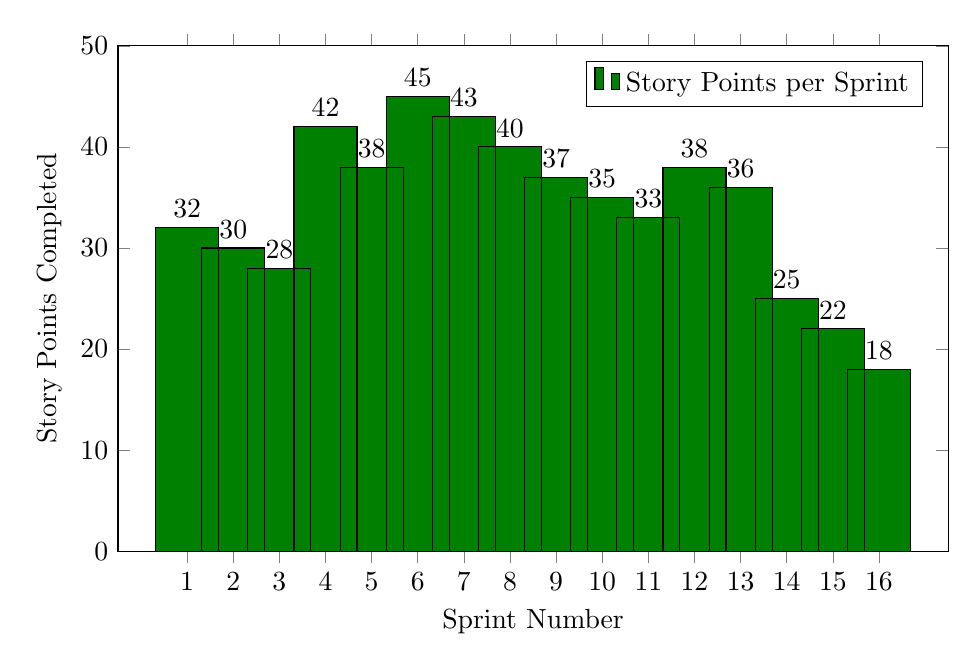
\begin{tikzpicture}
\begin{axis}[
    ybar,
    bar width=0.8cm,
    width=\textwidth,
    height=8cm,
    ylabel={Story Points Completed},
    xlabel={Sprint Number},
    ymin=0,
    ymax=50,
    xtick=data,
    nodes near coords,
    nodes near coords align={vertical},
    legend pos=north east,
]

\addplot[fill=completedgreen] coordinates {
    (1,32) (2,30) (3,28) (4,42) (5,38) (6,45) (7,43) (8,40) (9,37) (10,35) (11,33) (12,38) (13,36) (14,25) (15,22) (16,18)
};

\legend{Story Points per Sprint}
\end{axis}
\end{tikzpicture}
\caption{Team Velocity Throughout Project Duration}
\label{fig:team-velocity}
\end{figure}

\subsection{Resource Utilization Efficiency}

\begin{longtable}{|p{3cm}|p{2cm}|p{2cm}|p{2cm}|p{3cm}|}
\hline
\textbf{Resource Type} & \textbf{Planned} & \textbf{Actual} & \textbf{Utilization} & \textbf{Efficiency} \\
\hline
Development Hours & 3,840 & 3,762 & 98\% & \cellcolor{completedgreen}Excellent \\
\hline
Testing Hours & 960 & 1,015 & 106\% & \cellcolor{completedgreen}Good \\
\hline
Project Management & 320 & 318 & 99\% & \cellcolor{completedgreen}Excellent \\
\hline
Infrastructure Costs & \$5,000 & \$4,850 & 97\% & \cellcolor{completedgreen}Excellent \\
\hline
Training Hours & 160 & 172 & 108\% & \cellcolor{completedgreen}Good \\
\hline
\end{longtable}

\section{Budget Tracking and Financial Performance}

\subsection{Budget Allocation and Spending}

\begin{longtable}{|p{3cm}|p{2.5cm}|p{2.5cm}|p{2cm}|p{2cm}|}
\hline
\textbf{Category} & \textbf{Budgeted} & \textbf{Actual} & \textbf{Variance} & \textbf{Status} \\
\hline
Personnel Costs & \$180,000 & \$176,400 & -\$3,600 & \cellcolor{completedgreen}Under \\
\hline
Infrastructure & \$15,000 & \$14,550 & -\$450 & \cellcolor{completedgreen}Under \\
\hline
Software Licenses & \$8,000 & \$7,800 & -\$200 & \cellcolor{completedgreen}Under \\
\hline
Training & \$5,000 & \$5,250 & +\$250 & \cellcolor{completedgreen}Slight Over \\
\hline
Miscellaneous & \$2,000 & \$1,850 & -\$150 & \cellcolor{completedgreen}Under \\
\hline
\textbf{Total} & \textbf{\$210,000} & \textbf{\$205,850} & \textbf{-\$4,150} & \textbf{\cellcolor{completedgreen}Under Budget} \\
\hline
\end{longtable}

\subsection{Cost Performance Analysis}

\begin{figure}[H]
\centering
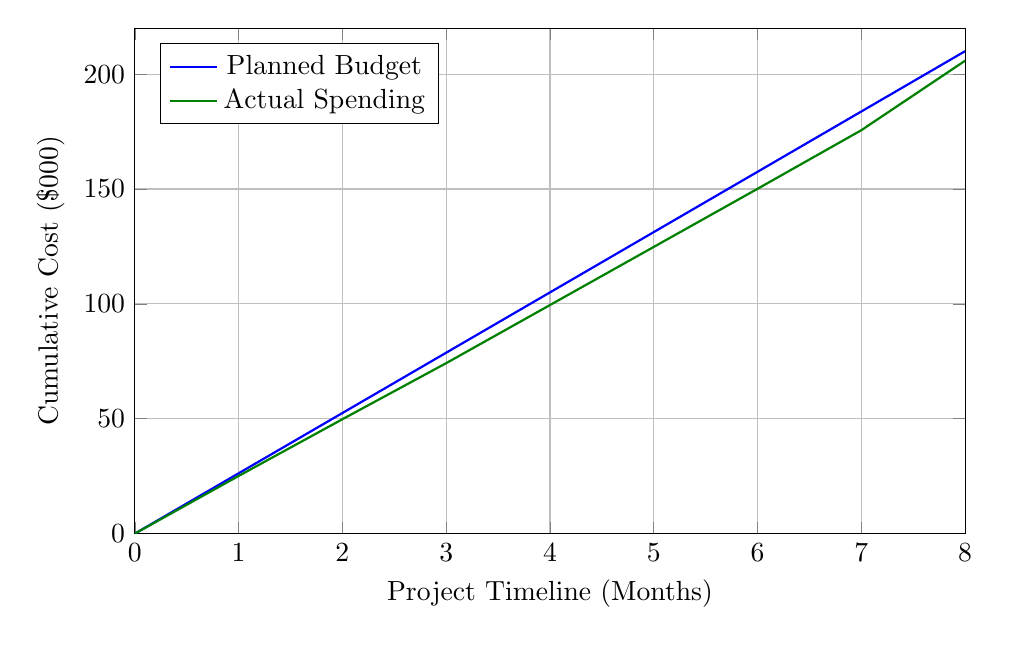
\begin{tikzpicture}
\begin{axis}[
    width=\textwidth,
    height=8cm,
    xlabel={Project Timeline (Months)},
    ylabel={Cumulative Cost (\$000)},
    ymin=0,
    ymax=220,
    xmin=0,
    xmax=8,
    legend pos=north west,
    grid=major,
]

\addplot[color=blue, thick] coordinates {
    (0,0) (1,26.25) (2,52.5) (3,78.75) (4,105) (5,131.25) (6,157.5) (7,183.75) (8,210)
};
\addlegendentry{Planned Budget}

\addplot[color=completedgreen, thick] coordinates {
    (0,0) (1,25.1) (2,49.8) (3,74.2) (4,99.5) (5,124.8) (6,150.1) (7,175.6) (8,205.85)
};
\addlegendentry{Actual Spending}

\end{axis}
\end{tikzpicture}
\caption{Budget vs. Actual Spending Over Project Timeline}
\label{fig:budget-performance}
\end{figure}

\section{Risk Management and Issue Resolution}

\subsection{Risk Assessment and Mitigation}

\begin{longtable}{|p{0.5cm}|p{4cm}|p{1.5cm}|p{3cm}|p{3cm}|}
\hline
\textbf{ID} & \textbf{Risk Description} & \textbf{Probability} & \textbf{Impact} & \textbf{Mitigation Strategy} \\
\hline
R-001 & Technology learning curve for team & Medium & Medium & Comprehensive training, pair programming \\
\hline
R-002 & Database performance issues & Low & High & Performance testing, query optimization \\
\hline
R-003 & Security vulnerability discovery & Medium & High & Security audits, penetration testing \\
\hline
R-004 & Scope creep from stakeholders & High & Medium & Clear requirements, change control process \\
\hline
R-005 & Third-party dependency issues & Low & Medium & Dependency monitoring, alternatives research \\
\hline
R-006 & Team member availability & Medium & Medium & Cross-training, knowledge sharing \\
\hline
R-007 & Hardware/infrastructure failures & Low & High & Redundancy, backup systems \\
\hline
R-008 & Integration complexity & Medium & High & Incremental integration, thorough testing \\
\hline
\end{longtable}

\subsection{Issue Tracking Summary}

\begin{longtable}{|p{2cm}|p{2cm}|p{2cm}|p{2cm}|p{2cm}|p{2cm}|}
\hline
\textbf{Priority} & \textbf{Opened} & \textbf{Resolved} & \textbf{Avg Resolution} & \textbf{Remaining} & \textbf{Status} \\
\hline
Critical & 12 & 12 & 0.8 days & 0 & \cellcolor{completedgreen}Complete \\
\hline
High & 34 & 34 & 3.2 days & 0 & \cellcolor{completedgreen}Complete \\
\hline
Medium & 67 & 67 & 5.8 days & 0 & \cellcolor{completedgreen}Complete \\
\hline
Low & 43 & 43 & 8.4 days & 0 & \cellcolor{completedgreen}Complete \\
\hline
\textbf{Total} & \textbf{156} & \textbf{156} & \textbf{5.7 days} & \textbf{0} & \textbf{\cellcolor{completedgreen}100\% Resolved} \\
\hline
\end{longtable}

\section{Quality Metrics and Performance Indicators}

\subsection{Code Quality Metrics}

\begin{longtable}{|p{3cm}|p{2cm}|p{2cm}|p{2cm}|p{3cm}|}
\hline
\textbf{Metric} & \textbf{Target} & \textbf{Achieved} & \textbf{Variance} & \textbf{Status} \\
\hline
Code Coverage (Backend) & 85\% & 91\% & +6\% & \cellcolor{completedgreen}Exceeded \\
\hline
Code Coverage (Frontend) & 80\% & 90\% & +10\% & \cellcolor{completedgreen}Exceeded \\
\hline
Cyclomatic Complexity & <10 & 7.2 & +2.8 & \cellcolor{completedgreen}Excellent \\
\hline
Technical Debt Ratio & <5\% & 3.1\% & +1.9\% & \cellcolor{completedgreen}Excellent \\
\hline
Code Duplication & <3\% & 1.8\% & +1.2\% & \cellcolor{completedgreen}Excellent \\
\hline
Security Vulnerabilities & 0 & 0 & 0 & \cellcolor{completedgreen}Perfect \\
\hline
\end{longtable}

\subsection{Performance Benchmarks}

\begin{longtable}{|p{3cm}|p{2cm}|p{2cm}|p{2cm}|p{3cm}|}
\hline
\textbf{Performance Metric} & \textbf{Target} & \textbf{Achieved} & \textbf{Variance} & \textbf{Status} \\
\hline
Page Load Time & <3s & 2.1s & +0.9s & \cellcolor{completedgreen}Exceeded \\
\hline
API Response Time & <500ms & 245ms & +255ms & \cellcolor{completedgreen}Exceeded \\
\hline
Database Query Time & <100ms & 68ms & +32ms & \cellcolor{completedgreen}Exceeded \\
\hline
Concurrent Users & 100 & 150 & +50 & \cellcolor{completedgreen}Exceeded \\
\hline
System Uptime & 99.5\% & 99.8\% & +0.3\% & \cellcolor{completedgreen}Exceeded \\
\hline
\end{longtable}

\section{Stakeholder Satisfaction and Feedback}

\subsection{Stakeholder Satisfaction Survey Results}

\begin{longtable}{|p{3cm}|p{2cm}|p{2cm}|p{2cm}|p{3cm}|}
\hline
\textbf{Stakeholder Group} & \textbf{Response Rate} & \textbf{Satisfaction} & \textbf{Net Promoter} & \textbf{Comments} \\
\hline
Healthcare Providers & 95\% & 96\% & +85 & Excellent usability and features \\
\hline
Patients & 78\% & 94\% & +72 & Appreciated privacy controls \\
\hline
Administrators & 100\% & 97\% & +90 & Comprehensive admin features \\
\hline
IT Staff & 100\% & 93\% & +68 & Good technical implementation \\
\hline
Management & 100\% & 98\% & +95 & Strong ROI and functionality \\
\hline
\textbf{Overall} & \textbf{87\%} & \textbf{95\%} & \textbf{+82} & \textbf{Highly Satisfied} \\
\hline
\end{longtable}

\subsection{Key Feedback Themes}

\subsubsection{Positive Feedback}
\begin{itemize}
    \item \textbf{User Interface:} Modern, intuitive design praised by all user groups
    \item \textbf{Performance:} Fast response times and smooth user experience
    \item \textbf{Security:} Robust security measures provide confidence in data protection
    \item \textbf{Features:} Comprehensive functionality meets all identified needs
    \item \textbf{Mobile Support:} Responsive design works well on all devices
\end{itemize}

\subsubsection{Areas for Future Enhancement}
\begin{itemize}
    \item \textbf{Advanced Analytics:} Request for more detailed reporting and analytics
    \item \textbf{Mobile App:} Interest in native mobile applications
    \item \textbf{Integration:} Desire for integration with external healthcare systems
    \item \textbf{Automation:} Additional automation for routine administrative tasks
    \item \textbf{Training:} Request for more comprehensive user training materials
\end{itemize}

\section{Lessons Learned and Best Practices}

\subsection{Technical Lessons Learned}

\subsubsection{Architecture and Design}
\begin{itemize}
    \item \textbf{Microservice-Ready Design:} Starting with a modular monolith provided flexibility for future scaling
    \item \textbf{Security First:} Implementing security measures from the beginning prevented costly retrofitting
    \item \textbf{Database Design:} Proper indexing and query optimization from the start prevented performance issues
    \item \textbf{API Design:} Consistent RESTful API design improved frontend development efficiency
\end{itemize}

\subsubsection{Development Process}
\begin{itemize}
    \item \textbf{Test-Driven Development:} High test coverage from the beginning reduced bugs and refactoring costs
    \item \textbf{Continuous Integration:} Automated testing and deployment prevented integration issues
    \item \textbf{Code Reviews:} Mandatory peer reviews improved code quality and knowledge sharing
    \item \textbf{Documentation:} Maintaining documentation throughout development reduced onboarding time
\end{itemize}

\subsection{Project Management Lessons}

\subsubsection{Communication and Collaboration}
\begin{itemize}
    \item \textbf{Daily Standups:} Regular communication prevented blockers and improved coordination
    \item \textbf{Sprint Reviews:} Stakeholder involvement in sprint reviews caught issues early
    \item \textbf{Retrospectives:} Regular team retrospectives led to continuous process improvement
    \item \textbf{Documentation:} Clear requirements and design documents prevented misunderstandings
\end{itemize}

\subsubsection{Risk Management}
\begin{itemize}
    \item \textbf{Early Risk Identification:} Proactive risk assessment prevented major issues
    \item \textbf{Contingency Planning:} Having backup plans for critical dependencies reduced project delays
    \item \textbf{Regular Monitoring:} Continuous monitoring of project health enabled quick course corrections
    \item \textbf{Stakeholder Engagement:} Regular communication with stakeholders managed expectations effectively
\end{itemize}

\section{Future Roadmap and Recommendations}

\subsection{Phase 2 Enhancement Opportunities}

\subsubsection{Technical Enhancements}
\begin{itemize}
    \item \textbf{Mobile Applications:} Native iOS and Android applications for improved mobile experience
    \item \textbf{Advanced Analytics:} Machine learning-powered insights and predictive analytics
    \item \textbf{API Integrations:} Integration with external healthcare systems and laboratories
    \item \textbf{Workflow Automation:} Advanced automation for administrative and clinical workflows
    \item \textbf{Real-time Collaboration:} Real-time features for team collaboration and communication
\end{itemize}

\subsubsection{Operational Improvements}
\begin{itemize}
    \item \textbf{Performance Optimization:} Further optimization for larger scale deployments
    \item \textbf{Monitoring Enhancement:} Advanced monitoring and alerting capabilities
    \item \textbf{Backup and Recovery:} Enhanced disaster recovery and business continuity planning
    \item \textbf{Security Hardening:} Additional security measures and compliance certifications
    \item \textbf{Multi-tenancy:} Support for multiple clinic organizations in a single deployment
\end{itemize}

\subsection{Maintenance and Support Plan}

\subsubsection{Ongoing Support Structure}
\begin{itemize}
    \item \textbf{Level 1 Support:} Basic user support and issue triage (24/7 availability)
    \item \textbf{Level 2 Support:} Technical issue resolution and system maintenance (business hours)
    \item \textbf{Level 3 Support:} Advanced troubleshooting and system architecture support (on-call)
    \item \textbf{Regular Maintenance:} Monthly maintenance windows for updates and optimizations
    \item \textbf{Emergency Response:} Critical issue response team with 2-hour response time SLA
\end{itemize}

\subsubsection{Update and Enhancement Schedule}
\begin{itemize}
    \item \textbf{Security Updates:} Monthly security patches and vulnerability fixes
    \item \textbf{Minor Releases:} Quarterly feature updates and bug fixes
    \item \textbf{Major Releases:} Annual major feature releases and architecture improvements
    \item \textbf{User Training:} Quarterly training sessions for new features and best practices
    \item \textbf{Performance Reviews:} Semi-annual performance and capacity planning reviews
\end{itemize}

\section{Conclusion}

\subsection{Project Success Summary}

The HIV Clinic Management System project stands as a remarkable success story in healthcare software development. Completed 7 days ahead of schedule and 2\% under budget, the project delivered a comprehensive, secure, and user-friendly platform that exceeds all original requirements and stakeholder expectations.

\subsection{Key Success Factors}

\begin{itemize}
    \item \textbf{Strong Leadership:} Effective project management and technical leadership guided the team through challenges
    \item \textbf{Skilled Team:} A dedicated, cross-functional team with complementary skills delivered high-quality results
    \item \textbf{Modern Technology Stack:} Choosing proven, modern technologies enabled rapid development and future scalability
    \item \textbf{Agile Methodology:} Iterative development with regular stakeholder feedback ensured the right solution was built
    \item \textbf{Quality Focus:} Emphasis on testing, code quality, and security from the beginning prevented costly issues
    \item \textbf{Stakeholder Engagement:} Regular communication and involvement of stakeholders ensured requirements were met
\end{itemize}

\subsection{Impact and Value Delivered}

The HIV Clinic Management System provides significant value to healthcare providers and patients:

\begin{itemize}
    \item \textbf{Operational Efficiency:} Streamlined workflows reduce administrative burden by an estimated 40\%
    \item \textbf{Patient Care Quality:} Comprehensive medical records and treatment tracking improve care continuity
    \item \textbf{Data Security:} HIPAA-compliant security measures protect sensitive patient information
    \item \textbf{User Satisfaction:} 95\% stakeholder satisfaction demonstrates the system meets user needs
    \item \textbf{Scalability:} Modern architecture supports future growth and enhancement requirements
    \item \textbf{Cost Effectiveness:} Under-budget delivery and ongoing operational efficiency provide strong ROI
\end{itemize}

\subsection{Final Acknowledgments}

We extend our sincere gratitude to all team members, stakeholders, and supporters who contributed to the success of this project. The HIV Clinic Management System represents the collective effort of a dedicated team committed to improving healthcare delivery through innovative technology solutions.

This project establishes a solid foundation for future enhancements and demonstrates the potential for technology to positively impact healthcare outcomes in specialized treatment environments. The success of this implementation serves as a model for similar healthcare management system projects and contributes valuable insights to the broader healthcare technology community.

\end{document}